
%Out of the 60 sites with preinstalled Infra-Red Camera Traps (IR CTs) I chose for my study, 56 were included in the analysis.
%19 of them remained unchanged through the whole study period as a control group. The remaining 37 were divided in two treatment groups that alternated on being equipped with an additional white LED CT in three month periods. The periods they were equipped with white LED are referred to in this section as LED (periods), and the periods without white LED are referred to as IR (periods). %AMkomm: metode

%TODO total number of active camera days included in the GLMM after trimming past 84 days.

The type of CT flash had an overall minor effect on detection rates.
In general, the control periods (which never had white flashes) had a somewhat lower detection rate than the IR and wLED periods.
%Between the experiment periods, I expected the IR periods to have the highest detection rate, but LED was somewhat higher for most species (see table \ref{tab:params}). %AMkomm: why?

There were a total of TK camera trapping days, which was unevenly distributed between the different periods and period types. Trimming the data according to median period length of IR periods (which was shorter than that of control and wLED periods) evened out the disproportions between the periods (see figure \ref{fig:active days}).

\begin{figure}
 \centering
	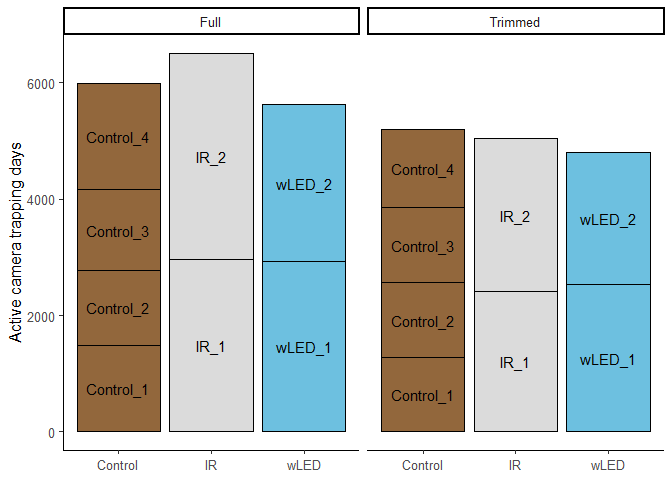
\includegraphics[scale=.9]{../R/glmm_sp_files/figure-html/active-days-3.png}
 \caption[Active camera days]
 {Active camera days %\par \small
 Number of active days per type of period, before and after trimming the data}
 \label{fig:active days}
\end{figure}




I will present detailed results of all the nine species included in my analyses in order most to least number of events, as shown in figure TK. % \ref{fig:events}
Each species is presented with a figure showing activity across time of day, a photo taken with a white LED CT of the species, %TODO (during night) 
an equivalence test, and a plot of the marginal means of the fixed effects in the GLMM model, showing the detection rates of all three types of periods (Control, IR and wLED) along a time axis.


\begin{figure}
 \centering
	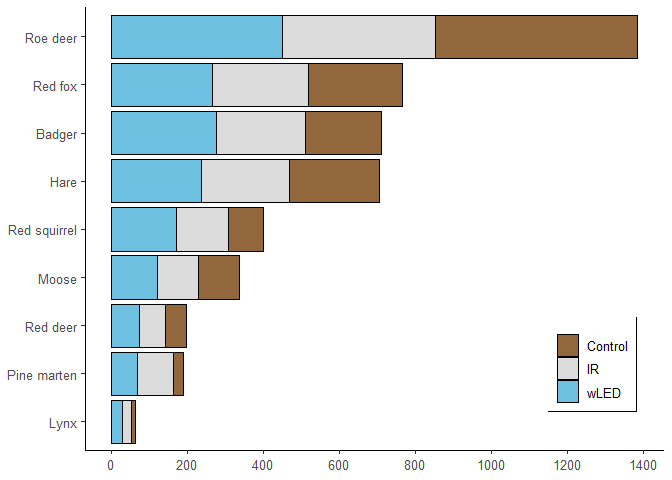
\includegraphics[scale=.9]{../R/glmm_sp_files/figure-html/events-1.png}
 \caption[Total number of events per species]
 {Total number of events per species}
 \label{fig:events}
\end{figure}


\begin{figure}
 \centering
	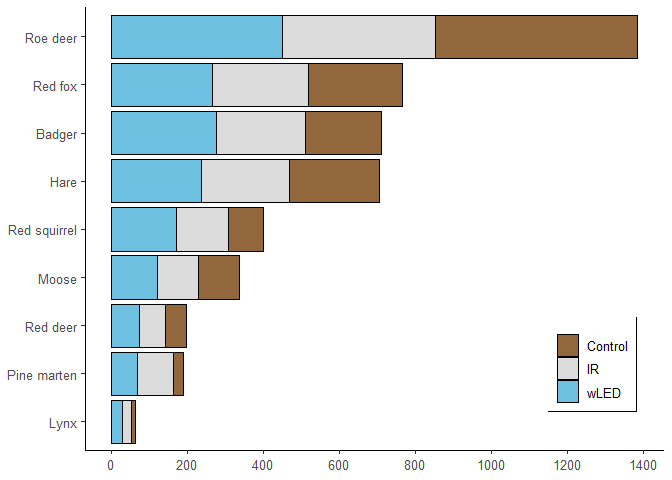
\includegraphics[scale=.9]{../R/glmm_sp_files/figure-html/events-1.png}
 \caption{Raw count and number of events per species}
\end{figure}




\subsection{Roe deer}

Roe deer was the most common species in my dataset, with a total number of 1709 events.
The species was detected at all times of day, with marked peaks of activity during the twilight hours.
Looking at the density curves in figure \ref{fig:raadyr}c, the overall pattern was consistent between the three types of periods (control, IR and wLED). 


There were almost 100 more photos of roe deer in the control group, than in the two treatment groups, but the control group also had more active camera trapping days.
IR periods also had more active CT days than the LED periods, which means that the detection rate was slightly higher with the white LED present.


This pattern is also demonstrated in figure \ref{fig:raadyr}a. 
However, the variation in the main effect of each period type (Control, IR and LED) were very large, and none of the periods were significantly different from each other.

Looking at figure \ref{fig:raadyr}b, the main effect of the IR and LED periods have a wide CI, which makes us unable to conclude on the groups' true effect sizes. IR is estimated to be within the Region of Practical Equivalence (ROPE), and LED is estimated to be outside, but the large variation still present in the data prevents a conclusion.
Considering the time variable, and it's interaction, all are within the ROPE, and the test tells us to accept it's practical equivalence to H0, namely that there is no effect.
Still, when interpreting a continuous variable as this, it is worth considering it's scale. I scaled my time variable to represent 10 day intervals, in order for the model to converge. That means the estimated effect of time since deployment is ten times larger than it would have been if it remained as 1 day intervals. Conversely, had I scaled it to represent the whole span of 84 days, the estimated effect and confidence interval would have been 8.4 times larger than what it is now ($\approx 0.4 $), and so would it's confidence interval. The equivalence test would be undecided on the effect of time since deployment.

Nevertheless, the control-group is what I am using as a reference point to what is normal. What I am interested in investigating is whether, and to what extent, the LED group deviates from the control group.

As mentioned, the main effect is non-significantly positive compared to both the control and the IR.
The same is true along the time axis. Both the slope for IR and LED are practically equivalent to the slope for control. Interesting to note, is however, that the slopes cross each other, which is what they would do if there is an effect of the LED, ie. that the IR periods counteract the effect of the LED periods.

Thus, I fail to reject the null hypothesis that white LED flash affects the detection rate of roe deer. Still, the variance is too large for me to be able to accept it. %relevant? need to make a comment on the disproportionate number of active days.


\subsection{Red fox}

After trimming data superceding a period length of 84 days,
the red fox was my second most common species with TK events.

The red fox was also active during the whole day, but with a more pronounced peak in the late evening continuing untill the break of day, as visualised in figure \ref{fig:rev}c.
The overall pattern was similar between each group (Control, IR, LED), which leads me to think that the overall effect of white LED was minor.
The GLMM explaining variation in detection rate of red fox had a substantial explanatory power (conditional R2 = 0.19), but the part related to the fixed effects alone (marginal R2) was just 0.001.
In other words, most of the explained variation in detection rate was due to seasonal changes and variation between the different camera sites captured in the random terms, and that the model was a worse fit for red fox than roe deer.

In a standard null hypothesis significance test (NHST) no parameters were significant.

Looking at figure \ref{fig:rev}a, the detection rate of red fox was generally lower in the control and IR-periods than in the LED-periods, and only the LED-periods showed a tendency towards a time-trend

Considering the equivalence test in figure \ref{fig:rev}b, the large variation in IR and LED hinders any decision on H0, although the estimate of LED (0.18) hints at a considerable attractant effect.

The slopes along the time axis (Time and Time * IR/LED) are practically equivalent to H0, ie. shows no sign of a substantial effect.


\subsection{SP}

SP was nth most common with n events.
SP was active during 
ie. most photos were taken during (night-time/daylight), as visualised in figure \ref{fig:SP}c.
The overall pattern was TK between each group (Control, IR, LED), which means that the overall effect of white LED ...
The GLMM explaining variation in detection rate of SP had a substantial explanatory power (conditional R2 = 0.xx), but the part related to the fixed effects alone (marginal R2) is just 0.00x.
In other words, most of the explained variation in detection rate was due to seasonal changes and variation between the different camera sites captured in the random terms.

In a standard null hypothesis significance test (NHST) the effect of white LED was TK significant, and TK parameters were considered significant.

Looking at figure \ref{fig:SP}a, the detection rate of SP was generally lower(?) in the control group than for the two treatment groups, and TK had the highest rate.
The slope for control group is approximately horizontal (?), and the slopes of the treatment groups...

Considering the equivalence test, which also is a visualisation of the numbers in \ref{tab:params}, the large variation in IR/LED...

The interaction with time since deployment is(n't) practically equivalent with the slope of Control.



Stikkord:
Results:
	-Total active days pre+post-trimming
	-Total count of sp events (also pre+post?)
-Overall detection rate pattern in all species
-Overall activity pattern in all species
-Density curves throughout the year, obs per (week/month)
-Intro to how each sp will be presented

Sp:
-Nth most common with n events,
	-at n of the 56 sites 
- activity pattern
	-compared to expected activity from literature (cite)
	-LED exposure (ie. activity during night
	(-activity-density with and without event-filter?)
-The model
	-TK parameter(s) was (non-|significant) in SNHT (see table \ref{tab:param})
	-Equivalence test says (mention 2nd gen p-value)
	-ggeffects plot shows...
-Conclusive sentence on species



\subsection{Model performance}

The models explaining variation and whatnot, mostly due to the random terms. This is to say that after having accounted for variations between camera sites, and seasonal fluctuations, there still was a lot of variation in the dataset left to explain, and the period-categories of "Control", "IR" and "LED" interacting with time since deployment didn't explain much of it.

Here I'd might go on to show a table with marginal and conditional R2 for all species. 

%Could also include a comparison of only fixed, only random and full mixed effect models, but that needs to come after I've completed results for all species AND written most of my discussion. Time is short!

method: \\
Using the performance package i checked various assumptions, and all held up %not true for some of the assumptions checked in the performance() %>% plot(), but I'm not sure all of them are that important.
%results, performance:
Overdispersion, zero-inflation and singularity all held up in every model. 




